%%%%%%%%%%%%%%%%%%%%%%%%%%%%%%%%%%%%%%%%%%%%%%%%%%%%%%%%%%%%%%%%%%
%%          mmm  mmmmmm mm   m        m    m mmmmmm mmm         %%
%%        m"   " #      #"m  #        #    # #        #         %%
%%        #   mm #mmmmm # #m #        #    # #mmmmm   #         %%
%%        #    # #      #  # #  """   #    # #        #         %%
%%         "mmm" #mmmmm #   ##        "mmmm" #mmmmm mm#mm       %%
%%                                                              %%
%%      Grundlagen der Elektrischen Netzwerke, UE               %%
%%      Gruppe 5, Team F                                        %%
%%      Authors: Severin Wolf, Maximilian Seidler.              %%
%%%%%%%%%%%%%%%%%%%%%%%%%%%%%%%%%%%%%%%%%%%%%%%%%%%%%%%%%%%%%%%%%%
% Note für Severin:
% mathe in latex glieder ich so:
%
% \[ <one line equation> /]
%
% \begin{equation}
%       numbered one line equation
% \end{equation}
%
% \begin{align*}
%       multi line equations (use \\ for linebreak and & to align)
% \end{align*}
%
% \begin{align}
%       numbered multi line equations
% \end{align}
%
\documentclass[a4paper]{article}
\usepackage{amsmath}
\usepackage[utf8]{inputenc}
\usepackage[T1]{fontenc}
\usepackage[english]{babel}
\usepackage{geometry}
\usepackage{graphicx}
\usepackage{tikz}
\geometry{a4paper,left=3cm,right=2cm, top=2cm, bottom=2cm} 
\usepackage[EFvoltages, european, straightvoltages]{circuitikz}

%tikz
\ctikzset{resistor = european}
\usetikzlibrary{decorations.pathreplacing}

%no paragraph indent
\setlength{\parindent}{0pt}

%for math, that does not fit
\renewcommand*{\arraystretch}{1.3}
\newcommand\scalemath[2]{\scalebox{#1}{\mbox{\ensuremath{\displaystyle #2}}}}

\newcommand\blfootnote[1]{%
	\begingroup
	\renewcommand\thefootnote{}\footnote{#1}%
	\addtocounter{footnote}{-1}%
	\endgroup
}

\begin{document}
\pagestyle{empty} \enlargethispage*{25cm}\samepage{
\vspace*{-3cm}
\begin{center}
\begin{minipage}[!h]{16cm}
\hspace*{0.2cm}

\includegraphics[width=3.3cm]{./Figures/igte_logo}
\begin{tabular}{p{8cm}}
\vspace{0.5cm}
\centering{
\Large Institut für Grundlagen und Theorie der Elektrotechnik\\
Technische Universität Graz\\
~\\}
\end{tabular}

\includegraphics[width=3.3cm]{./Figures/TUG_logo}
\end{minipage}
		\Large
		\textbf{Fundamentals of electrical networks} \vspace*{0.5cm}\\
		\textbf{1. Homework}\\
		Modified node voltage method \\
		\vspace*{0.5cm}
		\large
	        Team F: \quad Severin Wolf, \quad Maximilian Seidler \\
		14-17 March 2021
\end{center}

\tableofcontents
\listoffigures
\clearpage

\vspace*{0.6cm}

\section{Assignment 1}
	
	%%%%%%%%%%%%%%%%%%%%%%%%%%%%%%%%%%%%%%%%%%%%%%%%%%%%%%%%%%%%%%%%%%%%
	%%%%%%%%%%%%%%%%%%%%%%%%%%%%%%%%%%%%%%%%%%%%%%%%%%%%%%%%%%%%%%%%%%%%	
   Consider the following circuit depicted in figure \ref{fig:circuit_assignment1}. The voltage source
   $U_{S3}$ is a \textbf{current-controlled voltage source}. Use the modified node-voltage method
   (solve the circuit without a source transformation) to analyze the given circuit.

\begin{enumerate}
   \item Mark the current and the voltage across every element in the given circuit. Furthermore, add
   essential nodes important for solving this problem with the modified node voltage method and mark
   those too. \textbf{Use the given reference node} and mark all node voltages. Use Kirchhoff's
   current law to find the nodal equations in every node, except the given reference node, and derive
   the \textbf{node voltage} equations (\textbf{step-by-step}).  (1p)
		
   \item Define additonal conditions needed in order to solve the circuit. Write the system of
   equations in matrix form $\textbf{A} \cdot \textbf{x} = \textbf{b}$. (1p)
		
   \item Use Matlab to solve the system of equations given in matrix form. \textbf{Calculate the
   values of the node voltages, the unknown currents across the voltage sources, the value of the
   controlled voltage source $\mathbf{U_{S3}}$ and the current and voltage drop across every
   resistor}. The Matlab code, the calculations and the calculated results should be in your
   protocol. (1p)
		
   \item Calculate the power of every element in the circuit. All individual powers summed up with the
   correct sign must equal zero. (1p)
		
   \item Simulate the circuit in a suitable simulation- software (LTSPICE, PSPICE, ...) in order to
   verify your calculated results. Don't forget to add the simulation results to the protocol. (1p)
\end{enumerate}

	\subsection*{values:}
	$R_1 = 2\Omega$ \qquad $R_2 = 4\Omega$ \qquad $R_3 = 8\Omega$ \qquad $R_4 = 3\Omega$  \\
	$I_{s1} = 0.6A$ \qquad $U_{s2} = 4V$  \qquad $U_{s3} = \alpha \cdot I_{R_3}$ \qquad  $\alpha = 5$ 

\begin{figure}[h!] \centering    
\begin{circuitikz}%[scale = 0.5, transform shape]
      %Is_1
      \draw (0,0) to[I, i=$I_{S1}$, color=red]          (0,3);
      %n_1
      \draw (0,6) to[short]                             (6,6);
      %R_2
      \draw (3,6) to[R, *-*, l=$R_2$]                   (3,3);
      %R_1
      \draw (3,3) to[R, -*, l=$R_1$]                        (6,3);
      %Us_2
      \draw (0,3) to[V, v=$U_{s2}$, color=blue]         (3,3);
      %R_3
      \draw (3,3) to[R, -*, l=$R_3$, i=$I_{R3}$]        (3,0);
      %R_4
      \draw (0,3) to[R, *-, l=$R_4$]                        (0,6);
      %Controlled Us_3
      \draw (6,6) to[cvsource, v=$U_{s3}$, color=blue]  (6,3);
      %ref node
      \draw (0,0) to[short]                             (3,0);
      %grnd
      \draw (0,0) to (0,0) node[ground]{};
      %nodes
      \node[above]              (n_1) at (3,6) {$n_1$};
      \node[left]               (n_2) at (0,3) {$n_2$};
      \node[above, xshift=3mm]  (n_3) at (3,3) {$n_3$};
      \node[below]              (n_4) at (6,3) {$n_4$};
      \node[below] (ref) at     (3,0) {reference node};
\end{circuitikz}
\caption{Given circuit for assignment 1}
\label{fig:circuit_assignment1}
\end{figure}
\blfootnote{Deadline: 18.03.2021- 9:00 \qquad presentation: group No. 1}
\newpage
\section{Solution}
\subsection{Analytical calculations}

\begin{figure}[h!] \centering    
\begin{circuitikz}%[scale = 0.5, transform shape]
      %R_1
      \draw (10,5) 
      to[short] (9,5)
      to[R, l=$R_1$, v=$U_{R_1}$]  (6,5)
      to[short, i=$I_{R1}$, color=red] (5,5);
      %R_2
      \draw (5,10)
      to[short] (5,9)
      to[R, l=$R_2$, v=$U_{R_2}$]  (5,6)
      to[short, i=$I_{R2}$, color=red] (5,5);
      %R_3
      \draw (5,5)
      to[short] (5,4)
      to[R, l=$R_3$, v=$U_{R_3}$]   (5,1)
      to[short, i=$I_{R3}$, color=red] (5,0);
      %R_4
      \draw (0,5)
      to[short] (0,6)
      to[R, l=$R_4$, v=$U_{R_4}$]  (0,9)
      to[short, i=$I_{R4}$, color=red] (0,10);
      %Is_1
      \draw (0,0)
      to[short] (0,1)
      to[I, v^=$U_{S1}$] (0,4)
      to[short, i=$I_{S1}$, color=red] (0,5);
      %Us_2
      \draw (0,5) 
      to[short, i<=$I_{S2}^?$, color=red] (1,5) 
      to[V, v=$U_{s2}$]  (4,5)
      to[short] (5,5);
      %Controlled Us_3
      \draw (10,10)
      to[short, i<=$I_{S3}^?$, color=red] (10, 9)
      to[cvsource, v=$U_{S3}$]  (10,6)
      to[short] (10,5);
      %n_1
      \draw (0,10) to[short]                             (10,10);
      %ref 
      \draw (0,0) to[short]                             (5,0);
      %grnd
      \draw (0,0) to (0,0) node[ground]{};
      %nodes
      \draw[color=blue] (5,10) ellipse (150pt and 12pt);
      \node[above, color=blue]  (n_1) at (5,10) {$n_1$};
      \draw[color=blue] (0,5) ellipse (25pt and 25pt);
      \node[below, xshift=2mm, color=blue]   (n_2) at (0,5) {$n_2$};
      \draw[color=blue] (5,5) ellipse (25pt and 25pt);
      \node[below, xshift=-2mm, color=blue]  (n_3) at (5,5) {$n_3$};
      \draw[color=blue] (10,5) ellipse (25pt and 25pt);
      \node[below, color=blue] (n_4) at (10,5) {$n_4$};
      \draw (2.5,0) ellipse (75pt and 12pt);
      \node[below] (ref) at (2.5,0) {ref};
      %node voltage arrows
      \draw[-{Latex[length=2mm]}, color=blue] (2, 9.5) -- (2, 0.5)
      node[pos=0.65, right] {$U_{n1}$};
      \draw[-{Latex[length=2mm]}, color=blue] (0.5, 4.2) -- (1.5, 0.5)
      node[pos=0.2, right] {$U_{n2}$};
      \draw[-{Latex[length=2mm]}, color=blue] (4.5, 4.2) -- (2.5, 0.5)
      node[pos=0.2, left] {$U_{n3}$}; 
      \draw[-{Latex[length=2mm]}, color=blue] (9.5, 4.2) -- (4, 0.5)
      node[pos=0.2, xshift=-2mm, left] {$U_{n4}$};
\end{circuitikz}
\caption{Network with currents and (node-) voltages}
\label{fig:circuit_labeled}
\end{figure}
Solving the given network with the modified node-voltage method. Therefore, we need an
additional node $n4$ between the current-source $S3$. We are starting by setting up 
$n-1$ node equations using Kirchhoff's current law.
\begin{align*}
   n_1: \quad&I_{R2}-I_{R4}-I_{S3}^? &= 0 \\
   n_2: \quad&-I_{S1} - I_{S2}^? + I_{R4} &= 0 \\
   n_3: \quad&I_{S2}^? - I_{R1} - I_{R2} + I_{R3} &= 0 \\
   n_4: \quad&I_{S3}^? + I_{R1} &= 0
\end{align*}

With the known source current $I_{S1}$ brought to the other side, we can set up a matrix, for those
equations. $\vec{n}\vec{I} = \vec{b}$, where $\vec{n}$ represents current positions and directions,
$\vec{I}$ contains all network currents and  $\vec{s}$ contains already known source-currents.
\begin{equation}
   \begin{pmatrix}
      0 & 1 & 0 & -1 & 0 & -1 \\
      0 & 0 & 0 & 1 & -1 & 0  \\
      -1 & -1 & 1 & 0 & 1 & 0 \\
      1 & 0 & 0 & 0 & 0 & 1  
   \end{pmatrix}
   \cdot
   \begin{pmatrix}
       I_{R1} \\ I_{R2} \\ I_{R3} \\ I_{R4} \\ I_{S2}^? \\ I_{S3}^? 
   \end{pmatrix}
   =
   \begin{pmatrix}
      0 \\ I_{S1} \\ 0 \\ 0  
   \end{pmatrix}
   \label{eqn:nodes}
\end{equation}
Now we express those unknown resistor currents as node-voltages divided by resistance.
\[
   I_{R1} = \frac{U_{n4} - U_{n3}}{R_1}, \quad I_{R_2} = \frac{U_{n1} - U_{n3}}{R_2}, \quad
   I_{R3} = \frac{U_{n3}}{R_3}, \quad I_{R4} = \frac{U_{n2} - U_{n1}}{R_4}
.\]

\newpage

Instead of using resistances $\frac{1}{R_i}$,  we substitute them for conductances
$G_{i}$. For future ease of calculations, we once again form a matrix equation. Note, that we do not know
the currents $I_{S2}^?$ and $I_{S3}^?$ yet, so we leave them for now.
\begin{equation}
   \begin{pmatrix}
      0 & 0 & -G_1 & G_1 & 0 & 0 \\
      G_2 & 0 & -G_2 & 0 & 0 & 0 \\
      0 & 0 & G_3 & 0 & 0 & 0 \\
      -G_4 & G_4 & 0 & 0 & 0 & 0\\
      0 & 0 & 0 & 0 & 1 & 0 \\
      0 & 0 & 0 & 0 & 0 & 1 
   \end{pmatrix}
   \cdot
   \begin{pmatrix}
      U_{n1} \\ U_{n2} \\ U_{n3} \\ U_{n4} \\ I_{S2}^? \\ I_{S3}^?
   \end{pmatrix}
   =
   \begin{pmatrix}
       I_{R1} \\ I_{R2} \\ I_{R3} \\ I_{R4} \\ I_{S2}^? \\ I_{S3}^? 
   \end{pmatrix}
   \label{eqn:currents}
\end{equation}
We substitute the vector $\vec{I}$ from equation (\ref{eqn:nodes}) with the matricies from above. 

\[
   \begin{pmatrix}
      0 & 1 & 0 & -1 & 0 & -1 \\
      0 & 0 & 0 & 1 & -1 & 0  \\
      -1 & -1 & 1 & 0 & 1 & 0 \\
      1 & 0 & 0 & 0 & 0 & 1  
   \end{pmatrix}
   \cdot
   \begin{pmatrix}
      0 & 0 & -G_1 & G_1 & 0 & 0 \\
      G_2 & 0 & -G_2 & 0 & 0 & 0 \\
      0 & 0 & G_3 & 0 & 0 & 0 \\
      -G_4 & G_4 & 0 & 0 & 0 & 0\\
      0 & 0 & 0 & 0 & 1 & 0 \\
      0 & 0 & 0 & 0 & 0 & 1 
   \end{pmatrix}
   \cdot
   \begin{pmatrix}
      U_{n1} \\ U_{n2} \\ U_{n3} \\ U_{n4} \\ I_{S2}^? \\ I_{S3}^?
   \end{pmatrix}
   =
   \begin{pmatrix}
      0 \\ I_{S1} \\ 0 \\ 0  
   \end{pmatrix}
\]
\hspace{2cm}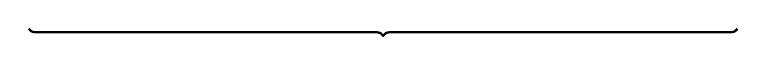
\begin{tikzpicture} 
   \draw[decoration={brace,mirror},decorate,thick]
      (0,0) -- (9,0);
\end{tikzpicture}

\begin{equation}
\begin{pmatrix}
   G_2 + G_4 & -G_4 & -G_2 & 0 & 0 & -1 \\
   -G_4 & G_4 & 0 & 0 & -1 & 0 \\
   -G_2 & 0 & G_1+G_2+G_3 & -G_1 & 1 & 0 \\
   0 & 0 & -G_1 & G_1 & 0 & 1 
\end{pmatrix}
\cdot
\begin{pmatrix}
   U_{n1} \\ U_{n2} \\ U_{n3} \\ U_{n4} \\ I_{S2}^? \\ I_{S3}^?
\end{pmatrix}
=
\begin{pmatrix}
   0 \\ I_{S1} \\ 0 \\ 0  
\end{pmatrix}
\label{eqn:nodes_currents}
\end{equation}

Just like that, we have our node voltage equations \,(\ref{eqn:nodes_currents}) in Form of $A \vec{x} = \vec{b}$, but we have 6 unknown
variables and only 4 equations to solve them. That's why we need two secondary conditions, to
compensate for the voltage sources $S_2$ and $S_3$.

\begin{align*}
   S_2: \quad &U_{n2} = U_{S2} \\ 
   S_3: \quad &U_{n1} - U_{n4} = U_{S3}
\end{align*}

So we add those as aditional rows to our admittance matrix $A$. Note, that the matrix $A$ is not
symetrical anymore, because we determined the source currents in the opposite direction of the
voltage arrows. 

\begin{equation}
\begin{pmatrix}
   G_2 + G_4 & -G_4 & -G_2 & 0 & 0 & -1 \\
   -G_4 & G_4 & 0 & 0 & -1 & 0 \\
   -G_2 & 0 & G_1+G_2+G_3 & -G_1 & 1 & 0 \\
   0 & 0 & -G_1 & G_1 & 0 & 1 \\ 
   0 & 0 & 1 & -1 & 0 & 0 \\
   1 & 0 & 0 & -1 & 0 & 0 
\end{pmatrix}
\cdot
\begin{pmatrix}
   U_{n1} \\ U_{n2} \\ U_{n3} \\ U_{n4} \\ I_{S2}^? \\ I_{S3}^?
\end{pmatrix}
=
\begin{pmatrix}
   0 \\ I_{S1} \\ 0 \\ 0 \\ U_{S2} \\ U_{S3} 
\end{pmatrix}
\label{eqn:nodes_currents_src}
\end{equation}

So far so good, but there is still one unknown variable, which is $U_{S3}$. This voltage is
proportional to the current $I_{R3}$. The Faktor between them is $\alpha$. With $U_{S3} = \alpha
I_{R3}$ and $I_{R3} = U_{n3}G_3$, we rearrange the equation $U_{n1} - U_{n4} = U_{S3}$ to
\[
   U_{n1} - U_{n4} - \alpha (U_{n3} G_3) = 0
.\]
We plug that into our matrix $A$ and get a solveable system of linear independent equations, $A
\vec{x} = \vec{b}$.
\begin{equation}
\begin{pmatrix}
   G_2 + G_4 & -G_4 & -G_2 & 0 & 0 & -1 \\
   -G_4 & G_4 & 0 & 0 & -1 & 0 \\
   -G_2 & 0 & G_1+G_2+G_3 & -G_1 & 1 & 0 \\
   0 & 0 & -G_1 & G_1 & 0 & 1 \\ 
   0 & 0 & 1 & -1 & 0 & 0 \\
   1 & 0 & -\alpha G_3 & -1 & 0 & 0 
\end{pmatrix}
\cdot
\begin{pmatrix}
   U_{n1} \\ U_{n2} \\ U_{n3} \\ U_{n4} \\ I_{S2}^? \\ I_{S3}^?
\end{pmatrix}
=
\begin{pmatrix}
   0 \\ I_{S1} \\ 0 \\ 0 \\ U_{S2} \\ 0
\end{pmatrix}
\label{eqn:final_matrix}
\end{equation}

\subsection{Matlab}
\subsubsection{Sourcecode}
\subsubsection{Console output}
\subsection{Numerical Results}
\subsubsection{Node Voltages}
\subsubsection{Unknown source currents/voltages}
\subsection{LTSpice Simulation}

\end{document}
